% Options for packages loaded elsewhere
\PassOptionsToPackage{unicode}{hyperref}
\PassOptionsToPackage{hyphens}{url}
%
\documentclass[
]{book}
\usepackage{lmodern}
\usepackage{amssymb,amsmath}
\usepackage{ifxetex,ifluatex}
\ifnum 0\ifxetex 1\fi\ifluatex 1\fi=0 % if pdftex
  \usepackage[T1]{fontenc}
  \usepackage[utf8]{inputenc}
  \usepackage{textcomp} % provide euro and other symbols
\else % if luatex or xetex
  \usepackage{unicode-math}
  \defaultfontfeatures{Scale=MatchLowercase}
  \defaultfontfeatures[\rmfamily]{Ligatures=TeX,Scale=1}
\fi
% Use upquote if available, for straight quotes in verbatim environments
\IfFileExists{upquote.sty}{\usepackage{upquote}}{}
\IfFileExists{microtype.sty}{% use microtype if available
  \usepackage[]{microtype}
  \UseMicrotypeSet[protrusion]{basicmath} % disable protrusion for tt fonts
}{}
\makeatletter
\@ifundefined{KOMAClassName}{% if non-KOMA class
  \IfFileExists{parskip.sty}{%
    \usepackage{parskip}
  }{% else
    \setlength{\parindent}{0pt}
    \setlength{\parskip}{6pt plus 2pt minus 1pt}}
}{% if KOMA class
  \KOMAoptions{parskip=half}}
\makeatother
\usepackage{xcolor}
\IfFileExists{xurl.sty}{\usepackage{xurl}}{} % add URL line breaks if available
\IfFileExists{bookmark.sty}{\usepackage{bookmark}}{\usepackage{hyperref}}
\hypersetup{
  pdftitle={An Exam P Study Guide},
  pdfauthor={Actuary Helper},
  hidelinks,
  pdfcreator={LaTeX via pandoc}}
\urlstyle{same} % disable monospaced font for URLs
\usepackage{longtable,booktabs}
% Correct order of tables after \paragraph or \subparagraph
\usepackage{etoolbox}
\makeatletter
\patchcmd\longtable{\par}{\if@noskipsec\mbox{}\fi\par}{}{}
\makeatother
% Allow footnotes in longtable head/foot
\IfFileExists{footnotehyper.sty}{\usepackage{footnotehyper}}{\usepackage{footnote}}
\makesavenoteenv{longtable}
\usepackage{graphicx}
\makeatletter
\def\maxwidth{\ifdim\Gin@nat@width>\linewidth\linewidth\else\Gin@nat@width\fi}
\def\maxheight{\ifdim\Gin@nat@height>\textheight\textheight\else\Gin@nat@height\fi}
\makeatother
% Scale images if necessary, so that they will not overflow the page
% margins by default, and it is still possible to overwrite the defaults
% using explicit options in \includegraphics[width, height, ...]{}
\setkeys{Gin}{width=\maxwidth,height=\maxheight,keepaspectratio}
% Set default figure placement to htbp
\makeatletter
\def\fps@figure{htbp}
\makeatother
\setlength{\emergencystretch}{3em} % prevent overfull lines
\providecommand{\tightlist}{%
  \setlength{\itemsep}{0pt}\setlength{\parskip}{0pt}}
\setcounter{secnumdepth}{5}
\usepackage{booktabs}
\usepackage{amsthm}
\makeatletter
\def\thm@space@setup{%
  \thm@preskip=8pt plus 2pt minus 4pt
  \thm@postskip=\thm@preskip
}
\makeatother
\usepackage[]{natbib}
\bibliographystyle{apalike}

\title{An Exam P Study Guide}
\author{Actuary Helper}
\date{2019-12-31}

\begin{document}
\frontmatter
\maketitle

{
\setcounter{tocdepth}{1}
\tableofcontents
}
\mainmatter
\hypertarget{an-introduction-to-set-theory}{%
\chapter{An Introduction to Set Theory}\label{an-introduction-to-set-theory}}

\hypertarget{defining-sets}{%
\section{Defining Sets}\label{defining-sets}}

Sets are collections of objects. Usually objects are placed inside curly braces and separated by commas. Here is the set with the numbers 1 and 2. We often give sets a name. This set is named ``A''. \[A=\{1,2\}\]

Objects inside the curly braces are called elements of the set. There is a special character that means ``is an element of''. Using our notation we can say that 1 is an element of A. \[1 \in A\]

We can also say that 3 is not an element of A by drawing a slash through our symbol.
\[3 \not\in A\]
We can define sets in a something called set-builder notation. Set builder notation is useful for infinite sets or sets that are hard to enumerate. Below are some examples.

We can define the even numbers as \(\{x | x \ is \  an \  even \ number\}\)

We can define hands of cards as \(\{x | x \ is \  a \ 5 \ element \ subset \ of \ a \ deck \ of \ cards\}\)

To read set builder notation we translate the ``\textbar{}'' as ``where''. So the real numbers are ``the set of x where x is a real number''.

\hypertarget{set-equality-and-subsets}{%
\section{Set Equality and Subsets}\label{set-equality-and-subsets}}

Sets are equal when they have the same elements. This means order doesn't matter in sets, \(\{1,2\} = \{2,1\}\) because they have the same elements. Also, \(\{1,1,2\} = \{1,2\}\) and we say that sets don't have duplicate elements because duplicate elements have no purpose.

A set is a subset of another set when it fits inside of it. There is a symbol that looks like \(\leq\) that means ``is a subset of''. For example \(\{1,2\} \subseteq \{1,2,3\}\). It is also true that any set is a subset of itself, so \(\{1,2\} \subseteq \{1,2\}\). In more precise terms \(A \subseteq B\) if and only if every element of A is also an element of B.

A common technique to prove that two sets are equal is to show that \(A \subseteq B\) and \(B \subseteq A\). This means there is no element in either set that does not belong to the other and the sets are equal.

\hypertarget{set-operations-and-venn-diagrams}{%
\section{Set Operations and Venn Diagrams}\label{set-operations-and-venn-diagrams}}

Just like you can add numbers together to make a new number, you can combine sets and make a new set. Let's define some sets.

\[S = \{1,2,3,4,5,6,7,8,9,10\} \\
 A = \{1,3,5,7\} \\
 B = \{2,3,4,5\}\]

\hypertarget{venn-diagram}{%
\subsection{Venn Diagram}\label{venn-diagram}}

There is a visual representation of sets called a Venn Diagram. In a Venn Diagram each set is represented by a circle. The sample space is usually represented by a large box that the circles are inside of.

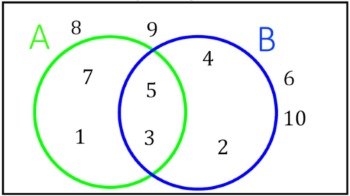
\includegraphics{Pictures/01-Sets/Venn.PNG}

\hypertarget{union}{%
\subsection{Union}\label{union}}

An element is in the union of A and B if it is in A, B, or A and B. The notation for this operation is \(A \cup B\) and it is pronounced ``A union B''. Here is the set that results from this union: \(A \cup B = \{1,2,3,4,5,7\}\)

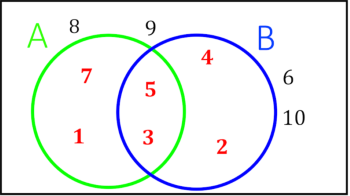
\includegraphics{Pictures/01-Sets/AUB.PNG}

\hypertarget{intersection}{%
\subsection{Intersection}\label{intersection}}

An element is in the intersection of A and B if it is in A and B. The notation for this operation is \(A \cap B\) and it is pronounced ``A intersect B''. Here is the set that results from this intersection: \(A \cap B = \{3,5\}\)

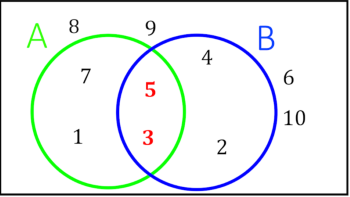
\includegraphics{Pictures/01-Sets/AcapB.PNG}

\hypertarget{complement}{%
\subsection{Complement}\label{complement}}

An element is in the complement of A if it is not in A, but is in the sample space. The notation for the complement of A is \(A^C\) and is pronounced ``A complement'' or ``the complement of A''. Here is the result of taking the complement of A: \(A^C = \{2,4,6,8,9,10\}\). Note that in general \((A^C)^C = A\).

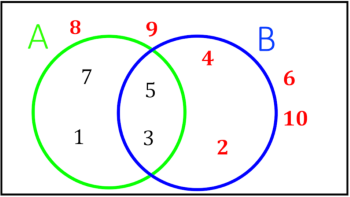
\includegraphics{Pictures/01-Sets/AC.PNG}

\hypertarget{set-difference}{%
\subsection{Set Difference}\label{set-difference}}

The set difference of A and B elements that are in A but not in B. The notation is either \(A \backslash B\) or \(A - B\) and is pronounced ``A minus B''. Here is the result of this set difference: \(A - B = \{7,1\}\). It is worth noting that \(A-B=A \cap B^C\) because the elements are in A and they are not in B.

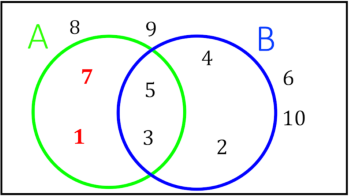
\includegraphics{Pictures/01-Sets/A-B.PNG}

\hypertarget{special-sets-and-identities}{%
\section{Special Sets and Identities}\label{special-sets-and-identities}}

\hypertarget{sample-space-and-empty-set}{%
\subsection{Sample Space and Empty Set}\label{sample-space-and-empty-set}}

The sample space is a type of special set because all other sets are subset of it. This leads to some commonsensical identities like \(A \cup S = S\) and \(A \cap S = A\). There is another special set called the empty set. This set has no elements. We could write it as \(\{\}\) but the common way to write this is \(\emptyset\). Some properties of the empty set are \(A \cup \emptyset = A\) and \(A \cap \emptyset = \emptyset\). It is also true that \(\emptyset^C = S\) and \(S^C = \emptyset\).

\hypertarget{de-morgans-laws}{%
\subsection{De Morgan's Laws}\label{de-morgans-laws}}

De Morgan's laws are formulas for the complement of a union or intersection of sets.
\[(A \cap B)^C = A^C \cup B^C \\
 (A \cup B)^C = A^C \cap B^C\]
One way of memorizing these formulas is that you bring the complement inside the parentheses to both sets and flip the union or intersection upside down.

Let's see if these laws make any sense. Let \(T\) be the set of tennis players and \(H\) be the set of hockey players. \((T \cap H)^C\) is the set of people that don't play both tennis and hockey. \(T^C \cup H^C\) is people that don't play tennis or they don't play hockey.If I don't play both sports then I either don't play tennis or I don't play hockey, so \((T \cap H)^C \subseteq T^C \cup H^C\). If I don't play tennis or I don't play hockey then it is true that I don't play both sports, so \(T^C \cup H^C \subseteq (T \cap H)^C\). This means that the sets are equal, ponder this for some time. A similar argument can be made for the complement of the union. If this is not convincing spend some time with a Venn diagram and see if you can get it to make sense.

\hypertarget{or-more-sets}{%
\subsection{3 or More Sets}\label{or-more-sets}}

\hypertarget{associativity}{%
\subsubsection{Associativity}\label{associativity}}

Just like you can add more than two numbers together you can take the intersection or union of more than two sets. For example \(\{1,2\} \cap \{2,3\} \cap \{3,4\} = \emptyset\). There are no elements in the intersection of these three sets because no number appears in all three sets, so this is the empty set. Intersections are associative, meaning \((A \cap B) \cap C= A \cap (B \cap C)\), so it doesn't matter what order you take a group of intersections in. Unions are also associative, \((A \cup B) \cup C= A \cup (B \cup C)\).

\hypertarget{messy-venn-diagrams}{%
\subsubsection{Messy Venn Diagrams}\label{messy-venn-diagrams}}

You can draw a Venn diagram for three sets with three circles. It gets a little complicated. I wouldn't bother drawing a Venn diagram for 4 sets.

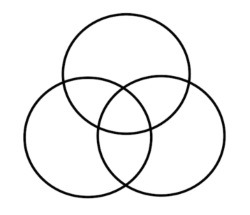
\includegraphics{Pictures/01-Sets/Venn3.PNG}
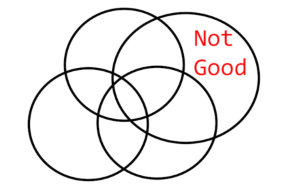
\includegraphics{Pictures/01-Sets/Venn4.PNG}

\hypertarget{distributive-property}{%
\subsubsection{Distributive Property}\label{distributive-property}}

If you mix together unions and intersections in an expression it isn't associative. Can you think of an example?
\[A \cap (B \cup C) \not= (A \cap B) \cup C\]
There are distributive formulas for situations like this.
\[A \cap (B \cup C) = (A \cap B) \cup (A \cap C) \\
 A \cup (B \cap C) = (A \cup B) \cap (A \cup C)\]
Because of this it is said that intersection distributes over unions, and that unions distribute across intersections. It is easier to remember these distributive formulas by comparing them to the way multiplication distributes over addition. \(a(b+c)=ab+ac\). Just pretend that the multiplication is an intersection and the addition is a union.

\hypertarget{counting}{%
\chapter{Counting}\label{counting}}

\hypertarget{size-of-a-set}{%
\section{Size of a set}\label{size-of-a-set}}

The set \(A = \{5,6\}\) has two elements. There is a notation to say the size of a set:
\[n(A) = 2\]
\(n\) is a function that takes in a set and outputs the number of elements in it:
\[n: Sets \to Whole \ Numbers\]
Let the sample space be \(S = \{1,2,3,4,5,6\}\). Since \(A=\{5,6\}\), \(A^C= \{1,2,3,4\}\) and \(n(A^C)=4\). There is a formula we can use for the size of the complement: \[n(A^C) = n(S) - n(A)=6-2=4\]
This is saying the size of the complement of a set is the size of the sample set minus the size of the set. I think this is pretty intuitive.

\hypertarget{principle-of-inclusion-exclusion}{%
\section{Principle of Inclusion-Exclusion}\label{principle-of-inclusion-exclusion}}

We define sets \(A\) and \(B\):
\[A = \{3,4,5\} \quad \quad B = \{4,5,6\}\]
We can see that \(A \cup B = \{3,4,5,6\}\) and \(n(A \cup B) = 4\).
Notice that \(n(A \cup B) \not = n(A) + n(B)\).

There is a special formula for the number of elements in a union called the principle of inclusion-exclusion.
\[n(A \cup B) = n(A) + n(B) - n(A \cap B)\]
We subtract \(n(A \cap B)\) from this expression because the elements of the intersection are counted twice - once in \(n(A)\), and once in \(n(B)\). Using the sets from earlier, \(A \cap B = \{4,5\}\). We can verify that the formula works by calculating \[n(A \cup B) = n(A) + n(B) - n(A \cap B) = 3 + 3 - 2 = 4\]

If the intersection of two sets is the empty set then the size of the union is the sum of the size of the sets.
\[A \cap B = \emptyset \iff n(A \cap B) = 0 \iff n(A \cup B) = n(A)+n(B)-0 = n(A)+n(B)\]
When two sets have no elements in common we call them \textbf{mutually exclusive}.

There is also a formula for the size of the union of three sets.
\[n(A \cup B \cup C) = n(A) + n(B) + n(C) - n(A \cap B)-n(B \cap C)-n(C \cap A) + n(A \cap B \cap C)\]
Consider how many times elements from each of the sections of a venn diagram with three sets are counted using the above formula. You should conclude that each element in \(A \cup B \cup C\) is counted exactly once.

\hypertarget{multiplication-principle}{%
\section{Multiplication Principle}\label{multiplication-principle}}

I have a red shirt and a blue shirt. I have a green hat, a pink hat, and a black hat. How many different shirt/hat combinations can I wear?

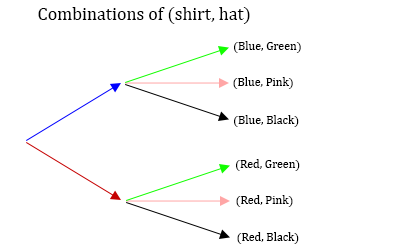
\includegraphics{Pictures/02-Counting/Tree.PNG}

The above diagram is an example of a \textbf{tree} diagram. The leaves (arrows with no arrows after them) of our tree represent the possible shirt/hat combinations. There are \(6\) possible shirt/hat combinations because there are \(2\) branches that each have \(3\) leaves which gives us \(2 \times 3 = 6\) total combinations. In general if there are \(m\) shirts and \(n\) hats there will be \(m \times n\) shirt/hat combinations because there will be \(m\) branches with \(n\) leaves. This generalizes to anything where you make two selections where the number of options in one of the selections does not depend on the other selection. For example the number of hats I can wear doesn't depend on which shirt I pick. If I decide that my pink hat is special and not to be worn with my red shirt then there are 5 combinations and the multiplication principle doesn't apply.

If I have \(4\) pairs of pants to choose from then there will be \(2 \times 3 \times 4\) shirt/hat/pant combinations. In general if you are making independent selections with \(a_1,a_2,...,a_n\) options, then the number of ways to make these selections is:
\[a_1 \times a_2 \times ... \times a_n=\displaystyle\prod_{k=1}^{n} a_k\]

\hypertarget{permutations}{%
\section{Permutations}\label{permutations}}

Permutations are all about rearranging things into ordered outcomes. For example, how many ways can we order the numbers in the set \(\{1,2,3\}\)? Let's draw a tree diagram to figure this out.

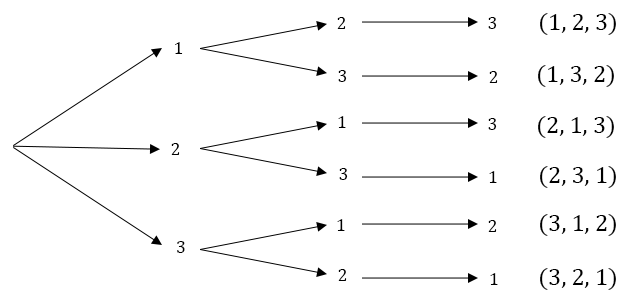
\includegraphics{Pictures/02-Counting/permute3large.PNG}

There are three options for our first selection, two options for our second selection, and one option for our third selection. The multiplication principle gives us 6 permutations of the set \(\{1,2,3\}\). Generally if \(n(A) = m\) there are \(m \times (m-1) \times ... \times 2 \times 1 = m!\) permutations of the set \(A\).

Here are some natural examples of permutations. How many possible outcomes are there in a three person race? We could imagine a set containing the different people and the outcomes of the race are the possible orders of the set. Some things not obviously involving order are permutation problems. If I bought three different chocolate bars how many ways can I give each of my three family members a chocolate bar? I think the natural way to do this is to use the multiplication principle to see that there are three options for the first chocolate bar I give away, two for the second, and one for the third. If I gave away all of the chocolates at the same time and there is no ordering it doesn't matter because I could have given the gifts away one at a time for the same set of possible outcomes.

Let's consider something more general. In a \(10\) person race how many possible outcomes are there for the top \(3\)? \(10\) people could have come in first place, there are \(9\) options for second once the first place is determined, and then \(8\) options for the third. The answer is then \(10 \times 9 \times 8=720\) using the multiplication principle. The general formula for the top \(k\) racers in an \(n\) person race is:
\[n \times (n-1) \times ... \times (n-k+1) = \frac{n!}{(n-k)!}\]
The situation for the top \(k\) racers in an \(n\) person race has it's own notation, \(P(n,k)\). \(P(n,k)\) is pronounced ``\(n\) permute \(k\)''.

\hypertarget{combinations}{%
\section{Combinations}\label{combinations}}

In permutations we consider how many possible orderings a subset of a certain size can have. What if we instead asked how many possible subsets there are of a certain size? For example, how many different ways can I pick \(2\) people from a group of \(3\) people? These problems are called combinations and the number of \(k\) element subsets of an \(n\) element set is \(C(n,k)\). An different notation that is more common is \(n \choose k\) and this is pronounced ``n choose k''. There is a relationship between permutations and combinations that we illustrate below.

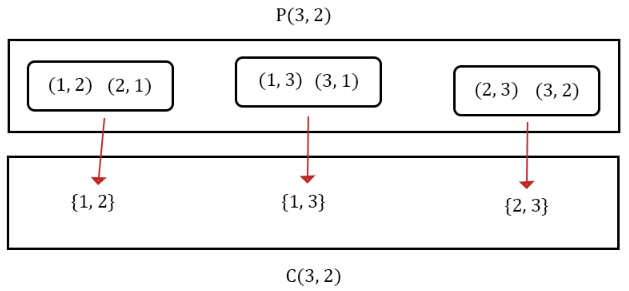
\includegraphics{Pictures/02-Counting/P(3,2)vsC(3,2).PNG}

For every set counted in \(C(3,2)\) there are two ordered pairs in \(P(3,2)\). Order doesn't matter in a combination, but it does in a permutation. If we select two people from a group of three there will be two permutations for each combination. If we select three people, there are six permutations per combination because there are six possible permutations of three people. In general we see that \(P(n,k) = C(n,k)\times k!\). Let's solve for \(C(n,k)\).

\(C(n,k) = \frac{P(n,k)}{k!} = \frac{n!}{k!(n-k)!}\)

\hypertarget{variations}{%
\section{Variations}\label{variations}}

Often a problem will involve using the multiplication principle with permutations and combinations. Consider the following:

There is a set of \(9\) distinct pigs. Three go to the market, three go to Arby's, and three go home. How many ways can this happen?

There are \(9 \choose 3\) ways to select the piggies for the market. After that selection is made there are \(6 \choose 3\) ways to select the piggies for Arby's. The remaining three piggies go home. The answer is then:
\[{9 \choose 3}\times{6 \choose 3} \times {3 \choose 3} = \frac{9!}{3!6!}\times \frac{6!}{3!3!} \times \frac{3!}{3!0!} = \frac{9!}{3!3!3!}\]
There is actually a general principle at work here. If we divide a set into mutually exclusive subsets then the number on the top is the size of the set and the numbers on the bottom are the size of the subsets.

\textbf{Is this true for dividing a set into two subsets? Why?}

A rephrasing of this question is ``How many ways can you rearrange the letters of `aaabbbccc'?'' To see that these questions are the same let each position of the letter be a piggy and assign the market, Arby's, and home to the letters a, b, and c.~Select positions in groups of three to assign the letters to.

Here is an example that combines permutations and combinations. ``How many ways could I rank my 10 favorite math problems from a list of 20 and then do 5 of them?'' There are \(P(20,10)\) possible rankings of my top 10 problems. There are \(10 \choose 5\) ways to choose from the selected problems. The answer is then:
\[P(20,10)\times{10 \choose 5} = 168,951,528,345,600\]

\hypertarget{probability-basics}{%
\chapter{Probability Basics}\label{probability-basics}}

\hypertarget{equiprob}{%
\section{Equally Likely Events}\label{equiprob}}

If we flip a coin it is said that heads and tails have the same probability because the percentage of both heads and tails tend toward \(50\%\) as the number of coin flips increases. Think of a \textbf{probability} as the percent of time an outcome occurs when many trials are performed. Here are the results of a simulation.

Number of Trials

Percent Heads

10

60\%

1,000

48.1\%

100,000

50.005\%

When we make a ``random selection'' it means that every possible selection has equal probability. For example, a randomly selected card from a deck of \(52\) cards has probability \(\frac{1}{52}\) of being a 2 of clubs.

When every possible outcome has equal probability, the formula for the probability of some subset of the outcomes is:

\[\frac{\text{Number of Selected Outcomes}}{\text{Number of Total Possible Outcomes}}\]

What is the probability of drawing 4 aces when we randomly select 5 cards from a deck? The number of ways to draw 4 aces is \({4 \choose 4} = 1\) because there are 4 aces and we must select all of them. There are 48 cards to select that are not aces which leads to \({48 \choose 1} = 48\) outcomes.

The number of ways to draw 4 aces is:
\[{4 \choose 4}{48 \choose 1} = 48\]

The number of ways to draw 5 cards is:
\[{52 \choose 5}\]

The answer is then:
\[\frac{{4 \choose 4}{48 \choose 1}}{{52 \choose 5}} = \frac{48}{2598960} = \frac{1}{54145}\]

\hypertarget{terminology}{%
\section{Terminology}\label{terminology}}

\hypertarget{sample-spaces-and-events}{%
\subsection{Sample Spaces and Events}\label{sample-spaces-and-events}}

In probability we talk about experiments, sample spaces, and events.

When we flip a coin or roll a die that is an \textbf{experiment}. Experiments have a set of possible outcomes that happen with some probability.

The set of all possible outcomes of an experiment is the \textbf{sample space}. When we flip a coin once the sample space is \(S=\{H,T\}\). When we flip a coin twice the sample space is \(S=\{HH,HT,TH,TT\}\).

\textbf{Events} represent a set of possible outcomes from an experiment. When we flip two coins there is an event for flipping two heads, \(E_\text{both heads}=\{HH\}\). There is also an event for not flipping two heads \(E_\text{not both heads}=\{HT,TH,TT\}\). An event is a subset of the sample space. It may represent a single outcome of our experiment, or it may represent several of the possible outcomes:
\[E \subseteq S\]

We can rewrite our formula for probabilities when all outcomes of an experiment are equally likely using \(n(E)\) for the number of selected outcomes.
\[\frac{\text{Number of Selected Outcomes}}{\text{Number of Total Possible Outcomes}} = \frac{n(E)}{n(S)}\]

\begin{center}\rule{0.5\linewidth}{0.5pt}\end{center}

\textbf{Example: Rolling Dice}

We roll two dice and want to calculate the probability that the dice sum to 4. Define the experiment, sample space, event, and calculate the probability of the event.

The experiment is rolling two dice.

The sample space has 36 elements, we can define it in set-builder notation:
\[\{(a,b)|a,b \in \{1,2,3,4,5,6\}\}\]
The event contains the elements of the sample space summing to 4.
\[E = \{(1,3),(3,1),(2,2)\}\]
The probability is
\[\frac{\text{Number of Selected Outcomes}}{\text{Number of Total Possible Outcomes}} = \frac{n(E)}{n(S)} = \frac{3}{36}=\frac{1}{12}\]

\begin{center}\rule{0.5\linewidth}{0.5pt}\end{center}

\hypertarget{probability-functions}{%
\section{Probability Functions}\label{probability-functions}}

There is a function called a probability function, denoted \(P\), that calculates the probability of an event. When we flip a coin twice the probability of getting a head and a tail is:
\[P(\{HT, TH\})=.5\]
For experiments where all outcomes are equally likely:
\[P(E) = \frac{n(E)}{n(S)}\]
A probability is between \(0\) and \(1\) because an event can't happen less than \(0\%\) of the time or more than \(100\%\) of the time. More formally, \(P\) is a function that takes an event as input and gives a number between \(0\) and \(1\) as output. In notation:
\[P:E \mapsto [0,1]\]

If we are being more mathematically rigorous, this rule about probabilities being between \(0\) and \(1\) is derived from some more basic assumptions and not intuition about the percentage of times something occurs. Let's talk about these basic assumptions.

\hypertarget{axiomsprob}{%
\subsection{Probability Axioms}\label{axiomsprob}}

There are three fundamental assumptions (called axioms) about probability functions from which our other laws are derived.

\textbf{First Axiom} - For an event \(E\), and probability function \(P\):
\[P(E) \geq 0\]
\textbf{Second Axiom} - For a sample space \(S\):
\[P(S)=1\]
\textbf{Third Axiom} - If \(E1, E2, ...En\) are \textbf{mutually exclusive} events:
\[P(\bigcup\limits_{i=1}^{\infty} E_{i})=P(E_1 \cup E_2 \cup...\cup En \cup...) = P(E1)+P(E2)+...+P(En)+...\]
For \textbf{two mutually exclusive} events events the third axiom is:
\[P(E_1 \cup E_2) = P(E_1)+P(E_2)\]

There are several formulas that are useful for this exam that can be derived from these axioms. We can derive the formula for the probability of the complement of an event:
\[P(A)+P(A^C) = P(A \cup A^C) = \ P(S) = 1 \ using \ Axioms \ 2 \ and \ 3\]
Since \(P(A^C)+P(A) = 1 \implies P(A^C) = 1-P(A)\).

Here are some useful formulas that can be derived from these axioms.
\[Complements: \ P(A^C) = 1 - P(A) \\
Upper \ Bound:P(A) \leq 1 \\
General \ Probability \ of \ 2 \ Unions: P(A \cup B) = P(A) + P(B) - P(A \cap B) \\
3 \ Unions: P(A \cup B \cup C) =  \\ P(A) + P(B) + P(C) - P(A \cap B)-P(B \cap C)-P(C \cap A) + P(A \cap B \cap C)\]

Notice that these formulas are the same as our formulas for the size of the set if we swap out \(P\) for \(n\) and \(1\) for \(n(S)\).

\begin{center}\rule{0.5\linewidth}{0.5pt}\end{center}

\textbf{Example: Coin Flipping and Axioms}

If we flip a coin, heads and tails are mutually exclusive events.
\[P(\{H\} \cup \{T\}) = P(\{H\})+P(\{T\}) = .5 + .5 = 1\]
We know that \(P(\{H\}), P(\{T\})=.5\) from our formula for equally likely events at the beginning of the chapter. Note that \(S = \{H\} \cup \{T\}\) so this example also illustrates that \(P(S)=1\).

\begin{center}\rule{0.5\linewidth}{0.5pt}\end{center}

\hypertarget{conditional-probability-and-independence}{%
\section{Conditional Probability and Independence}\label{conditional-probability-and-independence}}

Fluffy

Not Fluffy

Total

Cats

21

18

39

Dogs

35

26

61

Total

56

44

100

We make estimates about the overall population of pets using the results of a survey about pets. To do this we pretend that the pets in the survey represent the entire population of pets.

We can calculate the probability of a pet being fluffy using our formula for \protect\hyperlink{equiprob}{equally likely events}:
\[\frac{\text{Number of Fluffy Pets}}{\text{Total Number of Pets}} = \frac{n(\text{Fluffy})}{n(\text{Pets})} = \frac{56}{100}\]

We can calculate the probability of a pet being a fluffy cat as:
\[\frac{\text{Number of Fluffy Cats}}{\text{Total Number of Pets}} = \frac{n(\text{Fluffy} \cap \text{Cat})}{n(\text{Pets})} = \frac{21}{100}\]

We can also calculate the probability of a pet being fluffy, given that the pet is a cat:
\[\frac{\text{Number of Fluffy Cats}}{\text{Total Number of Cats}} = \frac{n(\text{Fluffy} \cap \text{Cat})}{n(\text{Cats})}=\frac{21}{39}\]
Calculating the probability of a pet being fluffy given that the pet is a cat is an example of conditional probability because in the denominator we do not include all of the possible pets, but only the cats. There is a special notation for conditional probabilities:
\[\text{Probability Pet is Fluffy given that Pet is a Cat} = P(\text{Pet is Fluffy}|\text{Pet is a Cat})\]
The general formula for conditional probabilities uses probabilities instead of set sizes. If all outcomes are equally likely either the probability or set size formula will give the same result:
\[\frac{P(\text{Fluffy} \cap \text{Cat})}{P(\text{Cat})} =  
\frac{n(\text{Fluffy and Cat})/n(\text{Pets})}{n(\text{Cat})/n(\text{Pets})} = \frac{n(\text{Fluffy}\cap\text{Cat})}{n(\text{Cat})}\]

\begin{center}\rule{0.5\linewidth}{0.5pt}\end{center}

\hypertarget{condprob}{%
\subsection{Conditional Probability Formulas}\label{condprob}}

The probability of event \(A\) given that event \(B\) has occurred is denoted \(P(A|B)\) and pronounced ``the probability of A given B''.
The general formula for this is \[P(A|B)=\frac{P(A \cap B)}{P(B)}\]

For experiments where all outcomes have equal probabilities \(P(A|B)\) can be calculated with set sizes. The derivation for forumla this was done in our example with fluffy cats. \[P(A|B)=\frac{n(A \cap B)}{n(B)}\]

We can calculate the probability of the intersection using the probability of the given event with the conditional probability. This formula is easiest to conceptualize if you imagine an event B happening with probability \(P(B)\) and then an event \(A\) happening with probability \(P(A|B)\). \[P(A|B) \times P(B) = P(A \cap B)\]

\begin{center}\rule{0.5\linewidth}{0.5pt}\end{center}

\hypertarget{independence}{%
\subsection{Independence}\label{independence}}

Events are independent if they do not influence each other. The first flip of a coin will not impact the second flip so these events are independent.

Let the event that the first card pulled without replacement from a deck is a jack be \(J_1\) and the event that the second card pulled is a jack is \(J_2\). If I pull a jack on my first try there will be less jacks in the deck for the second draw. The event \(J_1\) has an effect on \(J_2\) and these events are not independent.

\textbf{Definition of Independence}: Events \(A\) and \(B\) are said to be independent if \(P(A|B)=P(A)\).

This definition is equivalent to \(P(A \cap B) = P(A) \times P(B)\) after substitution with the \protect\hyperlink{condprob}{conditional probability formulas}. This identity has it's own name:

\textbf{Multiplication Rule for Independent Events}: If \(A\) and \(B\) are independent events then \(P(A \cap B) = P(A) \times P(B)\).

Let \(H_n\) be the event that the nth flip of a coin is heads so that \(H_2\) means the second coin flip is heads. The multiplication rule for independent events works for more than two events if all events are mutually independent so that \(P(H_1 \cap H_2 \cap H_3 \cap H_4)=P(H_1)\times P(H_2)\times P(H_3)\times P(H_4) = (\frac{1}{2})^4\).

\hypertarget{bayes-theorem}{%
\section{Bayes Theorem}\label{bayes-theorem}}

\hypertarget{bayes-theorem-intuition}{%
\subsection{Bayes Theorem Intuition}\label{bayes-theorem-intuition}}

Suppose 1\% of the population uses drugs. 98\% of drug users test positive on a drug test and 2\% of non-users test positive. What is the probability that a person testing positive for a drug test has used drugs?

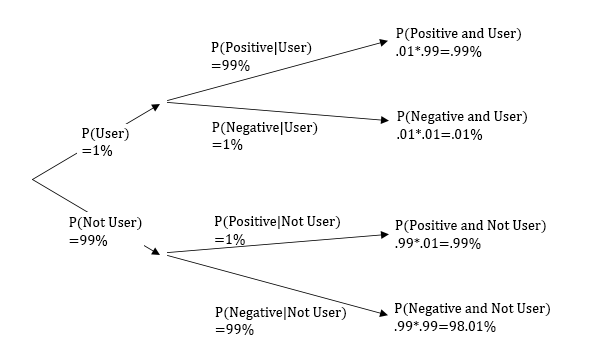
\includegraphics{Pictures/03-Probability/BayesTreeSmall.PNG}

Using the above tree diagram and the definition of conditional probability we calculate: \[P(User|Positive) = \frac{P(User \cap Positive)}{P(Positive)}= \\ 
\frac{P(User \cap Positive)}{P(Positive \cap Not \ User) + (Positive \cap User)} =\\  \frac{P(Positive|User) \times P(User)}{P(Positive|User) \times P(User)+P(Positive|Not \ User) \times P(Not \ User)} = \\
\frac{.0099}{.0099+.0099}=\frac{1}{2}\]

Let's explain these steps in more detail.

\hypertarget{law-of-total-probability}{%
\subsection{Law of Total Probability}\label{law-of-total-probability}}

In our calculation when we go from the first to the second line we use the identity \(P(Positive)=P(Positive \cap User)+P(Positive \cap Not \ User)\), but how do we know this is true?
\(Positive \cap User\) only contains drug users and \(Positive \cap Not \ User\) only contains non-users. These events are mutually exclusive so \(P(Positive \cap User)+P(Positive \cap Not \ User) = P((Positive \cap User) \cup (Positive \cap Not \ User))\) using our \protect\hyperlink{axiomsprob}{third probability axiom}. Using the distributive property for intersections with the identities
\[A^C \cup A = Sample \ Space, \quad A \cap (Sample \ Space) = A\]
we can see that:
\[(Positive \cap User) \cup (Positive \cap Not \ User) = Positive \cap (User \cup Not \ User) = \\ Positive \cap (Sample \ Space) = Positive\]
This is how we know that \(P(Positive)=P(Positive \cap User)+P(Positive \cap Not \ User)\).

There is a more general formulation of this known as the \textbf{law of total probability}:

\begin{center}\rule{0.5\linewidth}{0.5pt}\end{center}

Events \(A_1,A_2,...,A_n\) are said to be a \textbf{partition} of the sample space \(S\) if \(A_1 \cup A_2 \cup... \cup A_n=S\) and if for all \(i,j: \ A_i \cap A_j = \emptyset\). This just means that the sets \(A_1,A_2,...,A_n\) cover the whole set and there is no overlap between the sets.

If sets \(A_1,A_2,...,A_n\) partition \(S\) then for any event \(E\) we have \textbf{the law of total probability}:
\[P(E) = P(E \cap (A_1 \cup A_2 \cup ... \cup A_n)) = \\ P(E \cap A_1) + P(E \cap A_2) + ... + P(E \cap A_n) = \\ P(E|A_1) \times P(A_1) +...+ P(E|A_n) \times P(A_n)\]

Here is a visual:

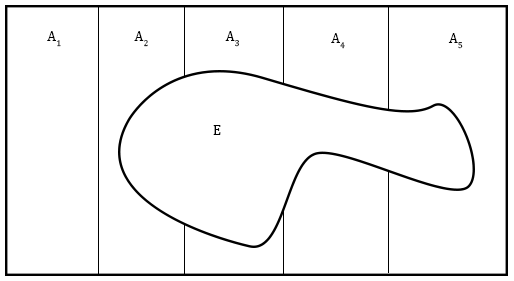
\includegraphics{Pictures/03-Probability/totalprob.PNG}

The proof of the law of total probability is outlined in our discussion of drug users.

\begin{center}\rule{0.5\linewidth}{0.5pt}\end{center}

\hypertarget{bayes-theorem-formula}{%
\subsection{Bayes Theorem Formula}\label{bayes-theorem-formula}}

\hypertarget{derivation-using-law-of-total-probability}{%
\subsubsection{Derivation Using Law of Total Probability}\label{derivation-using-law-of-total-probability}}

In our previous example every person is either a drug user or not so this partitions the sample space into two regions, \(User\) and \(Not \ User\). We can use the definition of conditional probability to say:
\[P(User|Positive)=\frac{P(User \cap Positive)}{P(Positive)}\]
We use the law of total probability in the denominator to expand it and convert all expressions of the form \(P(A \cap B)\) to expressions of the form \(P(B | A) \times P(A)\). The result is:
\[\frac{P(Positive|User) \times P(User)}{P(Positive|User) \times P(User)+P(Positive|Not \ User) \times P(Not \ User)}\]

\hypertarget{bayes-theorem-statement}{%
\subsubsection{Bayes Theorem Statement}\label{bayes-theorem-statement}}

For a partition \(A_1,A_2,...,A_n\) and event \(E\):
\[P(E|A_k) = \frac{P(E|A_k) \times P(A_k)}{P(E|A_1) \times P(A_1) +...+ P(E|A_n) \times P(A_n)}\]

\backmatter
  \bibliography{book.bib,packages.bib}

\end{document}
